\documentclass{beamer}
\mode<presentation>
\usepackage{amsmath,amssymb,mathtools}
\usepackage{textcomp}
\usepackage{gensymb}
\usepackage{adjustbox}
\usepackage{subcaption}
\usepackage{enumitem}
\usepackage{multicol}
\usepackage{listings}
\usepackage{url}
\usepackage{graphicx} % <-- needed for images
\def\UrlBreaks{\do\/\do-}

\usetheme{Boadilla}
\usecolortheme{lily}
\setbeamertemplate{footline}{
  \leavevmode%
  \hbox{%
  \begin{beamercolorbox}[wd=\paperwidth,ht=2ex,dp=1ex,right]{author in head/foot}%
    \insertframenumber{} / \inserttotalframenumber\hspace*{2ex}
  \end{beamercolorbox}}%
  \vskip0pt%
}
\setbeamertemplate{navigation symbols}{}

\lstset{
  frame=single,
  breaklines=true,
  columns=fullflexible,
  basicstyle=\ttfamily\tiny   % tiny font so code fits
}

\numberwithin{equation}{section}

% ---- your macros ----
\providecommand{\nCr}[2]{\,^{#1}C_{#2}}
\providecommand{\nPr}[2]{\,^{#1}P_{#2}}
\providecommand{\mbf}{\mathbf}
\providecommand{\pr}[1]{\ensuremath{\Pr\left(#1\right)}}
\providecommand{\qfunc}[1]{\ensuremath{Q\left(#1\right)}}
\providecommand{\sbrak}[1]{\ensuremath{{}\left[#1\right]}}
\providecommand{\lsbrak}[1]{\ensuremath{{}\left[#1\right.}}
\providecommand{\rsbrak}[1]{\ensuremath{\left.#1\right]}}
\providecommand{\brak}[1]{\ensuremath{\left(#1\right)}}
\providecommand{\lbrak}[1]{\ensuremath{\left(#1\right.}}
\providecommand{\rbrak}[1]{\ensuremath{\left.#1\right)}}
\providecommand{\cbrak}[1]{\ensuremath{\left\{#1\right\}}}
\providecommand{\lcbrak}[1]{\ensuremath{\left\{#1\right.}}
\providecommand{\rcbrak}[1]{\ensuremath{\left.#1\right\}}}
\theoremstyle{remark}
\newtheorem{rem}{Remark}
\newcommand{\sgn}{\mathop{\mathrm{sgn}}}
\providecommand{\abs}[1]{\left\vert#1\right\vert}
\providecommand{\res}[1]{\Res\displaylimits_{#1}}
\providecommand{\norm}[1]{\lVert#1\rVert}
\providecommand{\mtx}[1]{\mathbf{#1}}
\providecommand{\mean}[1]{E\left[ #1 \right]}
\providecommand{\fourier}{\overset{\mathcal{F}}{ \rightleftharpoons}}
\providecommand{\system}{\overset{\mathcal{H}}{ \longleftrightarrow}}
\providecommand{\dec}[2]{\ensuremath{\overset{#1}{\underset{#2}{\gtrless}}}}
\newcommand{\myvec}[1]{\ensuremath{\begin{pmatrix}#1\end{pmatrix}}}
\let\vec\mathbf

\title{MatGeo Presentation - Problem 2.9.15}
\author{EE25BTECH11064 - Yojit Manral}
\date{}

\begin{document}

\frame{\titlepage}
\begin{frame}{Question}
If the points $\vec{A}\brak{2,0}$, $\vec{B}\brak{6,1}$, and $\vec{C}\brak{p,q}$ form a triangle of area 12 square units(positive only) and
\begin{align}
    2p + q = 10
\end{align}
then find the values of p and q.
\end{frame}

\begin{frame}{Solution}
\begin{table}[h!]    
  \centering
  \begin{tabular}[12pt]{ |c| c|}
    \hline
    \textbf{Points} & \textbf{Name}\\ 
    \hline
	\myvec{7\\10} & Point $\Vec{A}$ \\
    \hline 
	\myvec{-2\\5} & Point $\Vec{B}$\\
    \hline
	\myvec{3\\4} & Point $\Vec{C}$\\
    \hline
\end{tabular}
  \caption{List of Points}
  \label{Table_1}
\end{table}
$\rightarrow$ Area of any $\triangle$ABC can be given by
\begin{align}
    Area(\text{ABC}) = \frac{1}{2} \left| \myvec{A & B & C\\1 & 1 & 1} \right| \notag
\end{align}
\end{frame}

\begin{frame}{Solution} 
$\rightarrow$ The area of the given $\triangle$ABC can be given by
\begin{align}
    Area(\text{ABC}) &= \frac{1}{2} \left| \myvec{2 & 6 & p\\0& 1 & q\\1 & 1 & 1} \right| \\
    2 \times Area(\text{ABC}) &= 2 \times \left| \myvec{1 & q\\1 & 1} \right| - 6 \times \left| \myvec{0 & q\\1 & 1} \right| + p \times \left| \myvec{0 & 1\\1 & 1} \right| \\
    &= 2(1-q) - 6(0-q) + p(0-1) \\
    &= 2 + 4q - p \\
    Area(\text{ABC}) &= 12 \\
    \left| 4q -p + 2 \right| &= 24 \\
    4q - p &= \pm 24 - 2
\end{align}
\end{frame}

\begin{frame}{Solution}
$\rightarrow$ From (1) and (8), we get
\begin{align}
    \myvec{2 & 1\\-1 & 4} \myvec{p\\q} &= \myvec{10\\\pm 24 - 2} \\
    \myvec{p\\q} &= \myvec{2 & 1\\-1 & 4}^{-1} \myvec{10\\ \pm 24 - 2} \\
    &= \frac{1}{9} \myvec{4 & -1\\1 & 2} \myvec{10\\ \pm 24 - 2} \\
    \myvec{p\\q} = \myvec{2\\6} &\text{ or } \myvec{p\\q} = \myvec{22/3\\ -14/3}
\end{align}
\end{frame}

\begin{frame}{Solution}
\begin{figure}[h!]
   \centering
   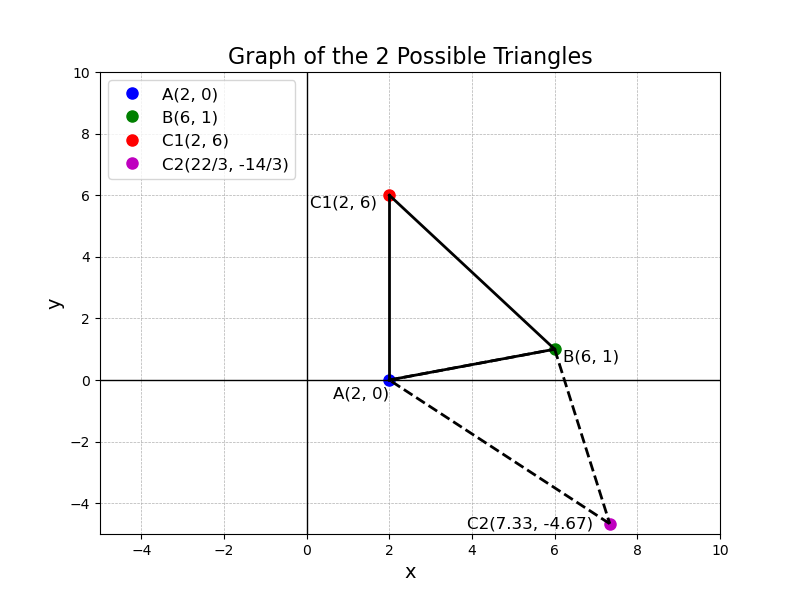
\includegraphics[width=0.8\linewidth]{figs/01.png}
   \caption{Plot of points and triangles}
   \label{Plot_1}
\end{figure}
\end{frame}

 % --------- CODE APPENDIX ---------
\section*{Appendix: Code}

% C program
\begin{frame}[fragile]{File: points.c}
\begin{lstlisting}[language=C]
#include <stdio.h>

int main() {
  FILE *fp;

  // -------------------
  // Question 2.9.15
  // -------------------


  fp = fopen("points.dat", "w");
  fprintf(fp, "%d,%d,%d\n", 2, 0, 0);  // A
  fprintf(fp, "%d,%d,%d\n", 6, 1, 0);  // B
  fprintf(fp, "%d,%d,%d\n", 2, 6, 0);  // C1
  fprintf(fp, "%d,%d,%d\n", 22/3, -14/3, 0);  // C2
  fclose(fp);
  return 0;
}
\end{lstlisting}
\end{frame}

% Python calling C
\begin{frame}[fragile]{File: call\_c.py}
\begin{lstlisting}[language=Python]
import subprocess

# Compile the C program
subprocess.run(["gcc", "points.c", "-o", "points"])

# Run the compiled C program
result = subprocess.run(["./points"], capture_output=True, text=True)

# Print the output from the C program
print(result.stdout)
\end{lstlisting}
\end{frame}

% Python plotting
\begin{frame}[fragile]{File: plot.py}
\begin{lstlisting}[language=Python]
import matplotlib.pyplot as plt

# Points
A = (2, 0)
B = (6, 1)
C1 = (2, 6)
C2 = (22/3, -14/3)

# Create the plot
fig, ax = plt.subplots(figsize=(8, 6))

# Plot the points A, B, C1, and C2
ax.plot(A[0], A[1], 'bo', label="A(2, 0)", markersize=8)
ax.plot(B[0], B[1], 'go', label="B(6, 1)", markersize=8)
ax.plot(C1[0], C1[1], 'ro', label="C1(2, 6)", markersize=8)
ax.plot(C2[0], C2[1], 'mo', label="C2(22/3, -14/3)", markersize=8)

# Connect the points A, B, and C1 to form the first triangle
ax.plot([A[0], B[0]], [A[1], B[1]], 'k-', lw=2)  # AB
ax.plot([B[0], C1[0]], [B[1], C1[1]], 'k-', lw=2)  # BC1
ax.plot([C1[0], A[0]], [C1[1], A[1]], 'k-', lw=2)  # C1A

# Connect the points A, B, and C2 to form the second triangle
ax.plot([A[0], B[0]], [A[1], B[1]], 'k--', lw=2)  # AB
ax.plot([B[0], C2[0]], [B[1], C2[1]], 'k--', lw=2)  # BC2
ax.plot([C2[0], A[0]], [C2[1], A[1]], 'k--', lw=2)  # C2A
\end{lstlisting}
\end{frame}

\begin{frame}[fragile]{File: plot.py}
\begin{lstlisting}[language=Python]
# Labels for the points
ax.text(A[0], A[1]-0.2, 'A(2, 0)', fontsize=12, ha='right', verticalalignment='top')
ax.text(B[0]+0.2, B[1], 'B(6, 1)', fontsize=12, ha='left', verticalalignment='top')
ax.text(C1[0]-0.3, C1[1], f'C1(2, 6)', fontsize=12, ha='right', verticalalignment='top')
ax.text(C2[0]-0.4, C2[1], f'C2({C2[0]:.2f}, {C2[1]:.2f})', fontsize=12, ha='right', verticalalignment='center')

# Set the axes limits
ax.set_xlim(-5, 10)
ax.set_ylim(-5, 10)

# Set labels and title
ax.set_xlabel('x', fontsize=14)
ax.set_ylabel('y', fontsize=14)
ax.set_title('Graph of the 2 Possible Triangles', fontsize=16)

# Show grid and customize
ax.grid(True, which='both', linestyle='--', linewidth=0.5)
ax.axhline(0, color='black',linewidth=1)
ax.axvline(0, color='black',linewidth=1)

# Show the legend
ax.legend(loc='upper left', fontsize=12)

# Show the plot
plt.show()
\end{lstlisting}
\end{frame}

\end{document}
